\documentclass[mathserif]{beamer}
\mode<presentation>
{
  \usetheme{Frankfurt}
  \setbeamercovered{transparent}
}

\setbeamertemplate{caption}[numbered]

\usepackage{bm}
\usefonttheme[onlymath]{serif}
\usepackage{mathrsfs}

\begin{document}


\title{Energy-Based Generative Adversarial Networks}

\author{Wenhao Yang
}
\institute{School of Mathematical Sciences

Peking University}
\begin{frame}
  \titlepage
\end{frame}

\date{}

\begin{frame}{Outline}
\tableofcontents
\end{frame}
\section{Introduction}
\subsection{Energy-Based Model}
\begin{frame}{Energy-Based Model}
\begin{itemize}
  \item Try to learn a function $f$, which maps each point of an input space to a single scalar.
  \begin{align}
    f: X\rightarrow R
  \end{align}
  where the scalar is called $``$energy$"$.
\end{itemize}
\begin{itemize}
  \item Ideal function $f$: the desired configuration gets assigned low energies while
  the incorrect ones are given high energies.
\end{itemize}
\begin{itemize}
  \item E.g:

  Supervised learning: low energy corresponds to correct label.

  Unsupervised learning: low energy corresponds to the data manifold.
\end{itemize}
\end{frame}
\subsection{Genrative Adversarial Networks}
\begin{frame}{Genrative Adversarial Networks}
GAN are combined with the following parts:
\begin{itemize}
  \item Discriminator
  \item Generator
  \item etc
\end{itemize}
\end{frame}
\section{Energy-Based Generative Adversarial Networks}
\begin{frame}{Energy-Based Generative Adversarial Networks}
  \begin{itemize}
    \item Discriminator is viewed as an energy function, without explicit probabilistic interpretation.
    \item Discriminator is trained to assign low energy values to regions of high data density.
    \item Generator is viewed as a trainable parameterized function that produces samples in regions
    of the space to which the generator assigns low energy.
  \end{itemize}
\end{frame}
\section{EBGAN Model}
\begin{frame}{EBGAN Model}
\begin{itemize}
  \item Notation:

  $p_{data}$: the underlying probability density of the distribution that produces the dataset.

  $G$: the generator which is trained to produce a sample $G(z)$

  $p_{z}$: A known distribution to provide a random vector $z$

  $D$: the discriminator which takes either real or generated samples and estimates the energy
  value $E\in R$
\end{itemize}
\begin{itemize}
  \item Objectie functional:

  Given a positive margin $m$, a data sample $x$ and a generated sample $G(z)$, defining the
  discriminator loss $\mathcal{L}_{D}$ and the generator loss $\mathcal{L}_{G}$:
  \begin{align}
    \mathcal{L}_{D}(x,z)&=D(x)+[m-D(G(z))]^{+}\\
    \mathcal{L}_{G}(z)&=D(G(z))
  \end{align}
\end{itemize}
\end{frame}
\begin{frame}{EBGAN Model}
  \begin{itemize}
    \item Define:
    \begin{align}
      V(G,D)&=\int_{x,z}\mathcal{L}_{D}(x,z)p_{data}(x)p_{z}(z)dxdz\\
      U(G,D)&=\int_{z}\mathcal{L}_{G}(z)p_{z}(z)dz
    \end{align}

    \item Aim: train the $D$ to minimize $V$ and
    train the $G$ to minimize $U$

    \item Nash equilibrium of the system is a pair $(G^{*},D^{*})$ that satisfies:
    \begin{align}
      V(G^{*},D^{*})\le V(G^{*},D)\hspace{6pt}\forall D\\
      U(G^{*},D^{*})\le U(G,D^{*})\hspace{6pt}\forall G
    \end{align}
  \end{itemize}
\end{frame}

\begin{frame}{EBGAN Model}
  \begin{theorem}
    If $(D^{*},G^{*})$ is a Nash equilibrium of the system,then $p_{G}\overset{a.s}{=}p_{data}$ and
    $V(D^{*},G^{*})=m$
  \end{theorem}
  \begin{theorem}
    Nash equilibrium of this system exists and is characterized by:

    (a) $p_{G}\overset{a.s}{=}p_{data}$

    (b) there exists a constant $\gamma\in[0,m]$ such that $D^{*}(x)\overset{a.s}{=}\gamma$
  \end{theorem}
\end{frame}
\begin{frame}{Auto-Encoders}
  The discriminator $D$ is structured as an auto-encoder:
  \begin{align}
    D(x)=||Dec(Enc(x))-x||
  \end{align}
  \begin{figure}
    \centering
    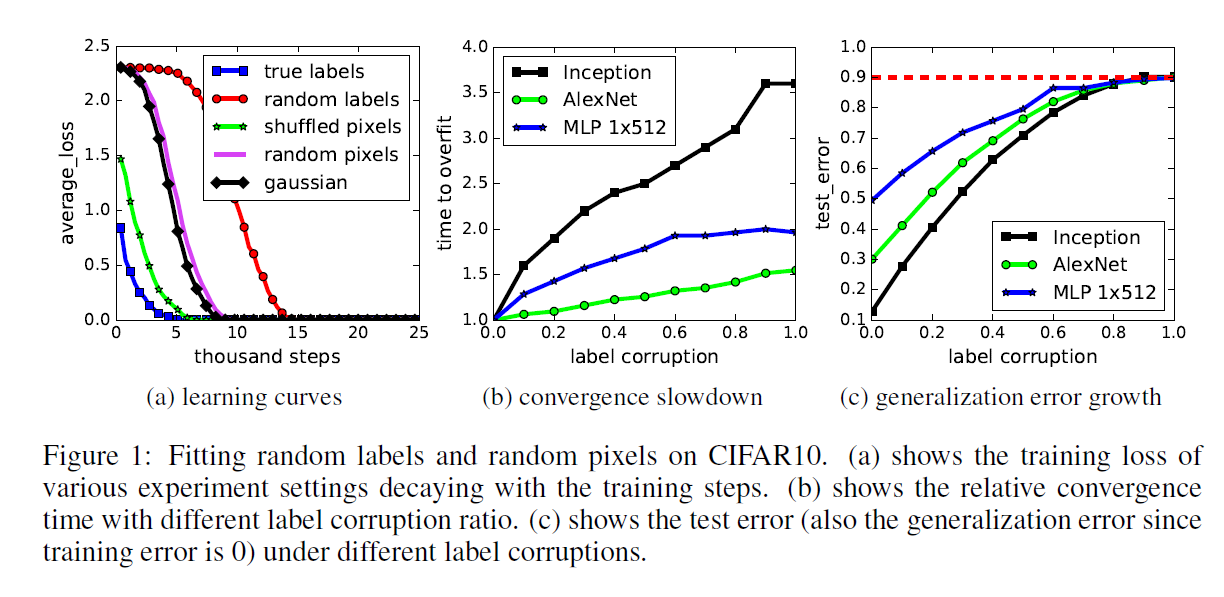
\includegraphics[scale=0.5]{fig/1.png}
    \label{}
  \end{figure}
\end{frame}
\begin{frame}{Auto-Encoders}
  Why Auto-Encoders?
  \begin{itemize}
    \item Offer a diverse targets for the discriminator

    \item Reconstruction loss will likely produce very different gradient directions within the minibatch, allowing for larger minibatch size without loss of efficiency.

    \item Given regularization, auto-encoders have the ability to learn an energy manifold without
    supervision or negative examples.
  \end{itemize}
  Problems:
  \begin{itemize}
    \item Auto-encoders may learn little more than an identity funcion, which means attributing low
    energy to the whole space.
  \end{itemize}
  Solution:
  \begin{itemize}
    \item Regularization: to give higher energy to points outside of the data manifold.
  \end{itemize}
\end{frame}

\begin{frame}{Auto-Encoders}
  Repelling Regularizer:
  \begin{itemize}
    \item Aim: to keep the model from producing samples that are clustered in one or a few modes of $p_{data}$
    \item Pulling-away(PT) effect:
    \begin{align}
      f_{PT}(S)=\frac{1}{N(N-1)}\sum_{i}\sum_{j\not=i}(\frac{S_{i}^{T}S_{j}}{||S_{i}||||S_{j}||})^{2}
    \end{align}
    where $S\in R^{s\times N}$ denotes a batch of sample representations taken from the encoder output layer.
    \item PT term is used in the generator loss but not discriminator loss
  \end{itemize}
\end{frame}
\section{Experiments Results}
\begin{frame}{Exhaustive Grid Search On MNITST}
\begin{figure}
  \centering
  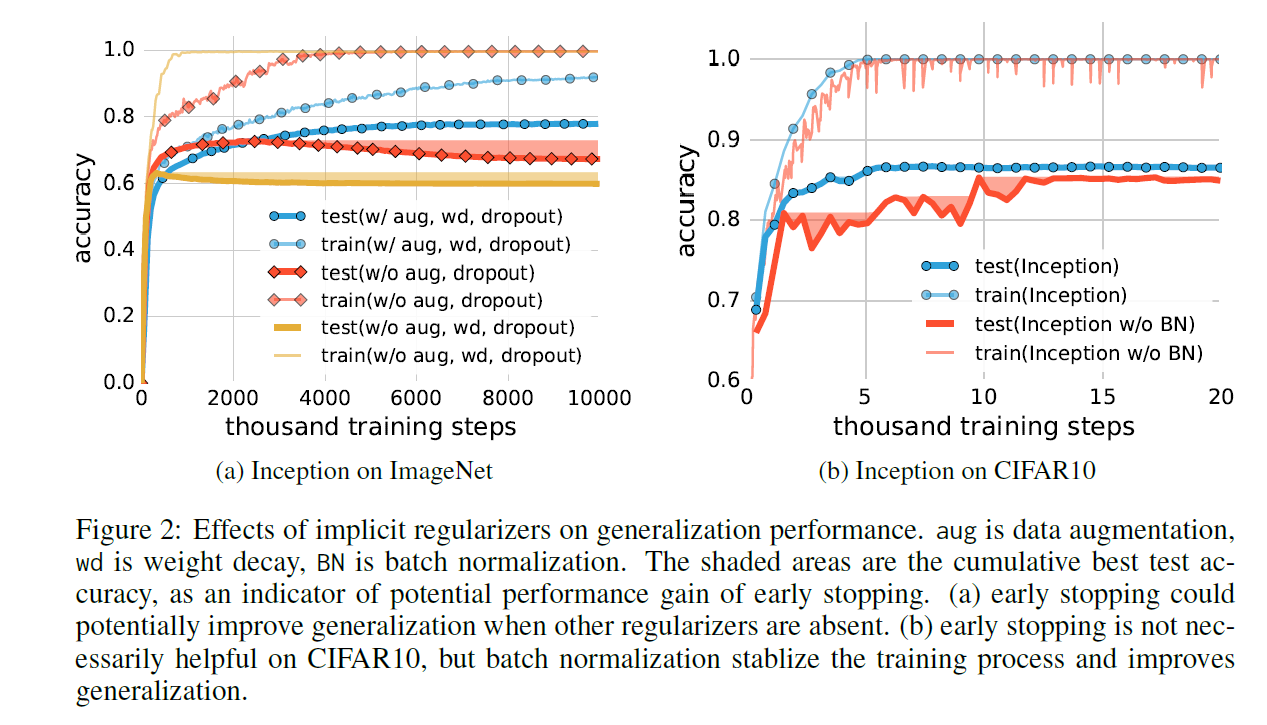
\includegraphics[scale=0.5]{fig/2.png}
  \label{}
\end{figure}
\end{frame}
\begin{frame}{Exhaustive Grid Search On MNITST}
\begin{figure}
  \centering
  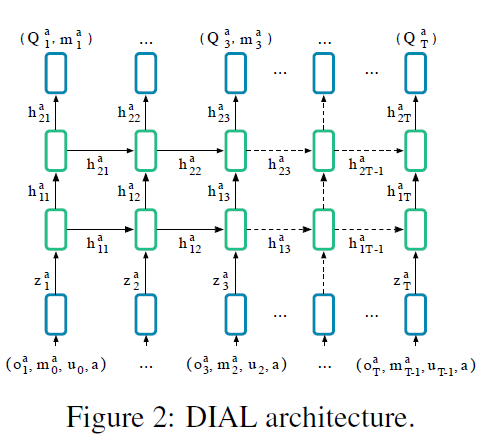
\includegraphics[scale=0.5]{fig/3.png}
  \label{}
\end{figure}
\end{frame}
\begin{frame}{Exhaustive Grid Search On MNITST}
\begin{figure}
  \centering
  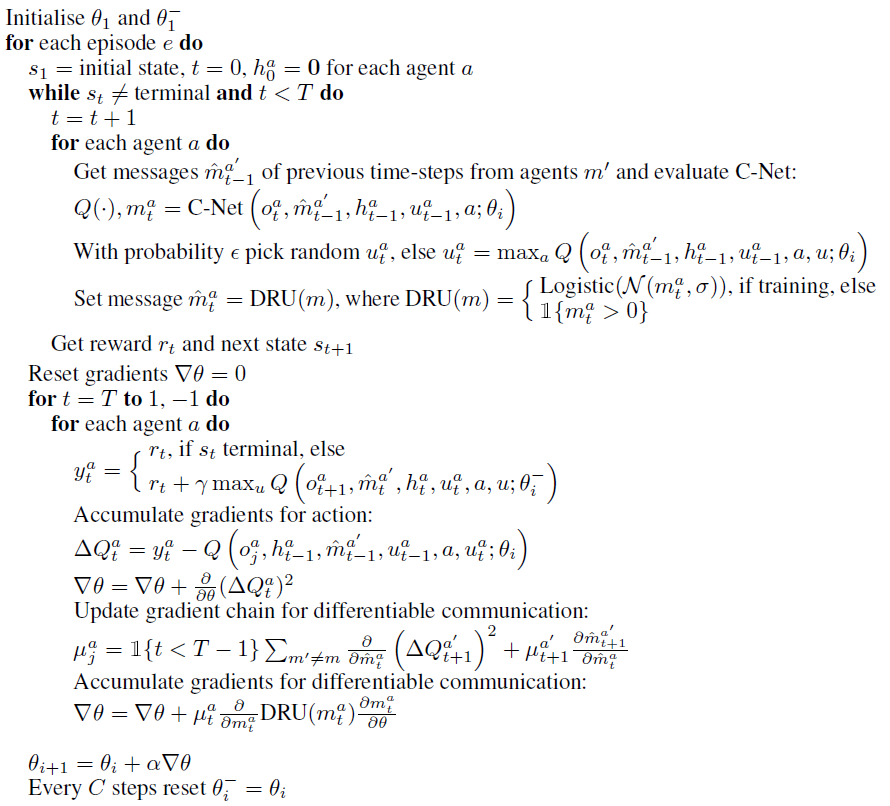
\includegraphics[scale=0.5]{fig/4.png}
  \label{}
\end{figure}
\end{frame}
\begin{frame}{Exhaustive Grid Search On MNITST}
\begin{figure}
  \centering
  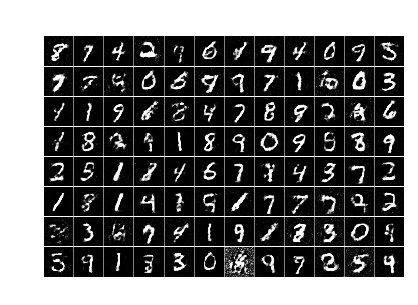
\includegraphics[scale=1]{fig/5.png}
  \caption{Best GAN model}
  \label{}
\end{figure}
\end{frame}
\begin{frame}{Exhaustive Grid Search On MNITST}
\begin{figure}
  \centering
  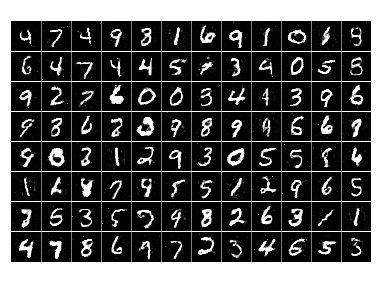
\includegraphics[scale=1]{fig/6.png}
  \caption{Best EBGAN model}
  \label{}
\end{figure}
\end{frame}\begin{frame}{Exhaustive Grid Search On MNITST}
\begin{figure}
  \centering
  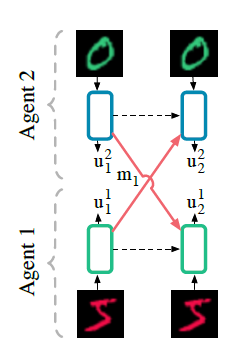
\includegraphics[scale=1]{fig/7.png}
  \caption{Best EBGAN-PT model}
  \label{}
\end{figure}
\end{frame}
\begin{frame}{Semi-Supervised Learning On MNIST}
Positioning a bottom-layer-cost LN into an EBGAN framework.
\begin{figure}
  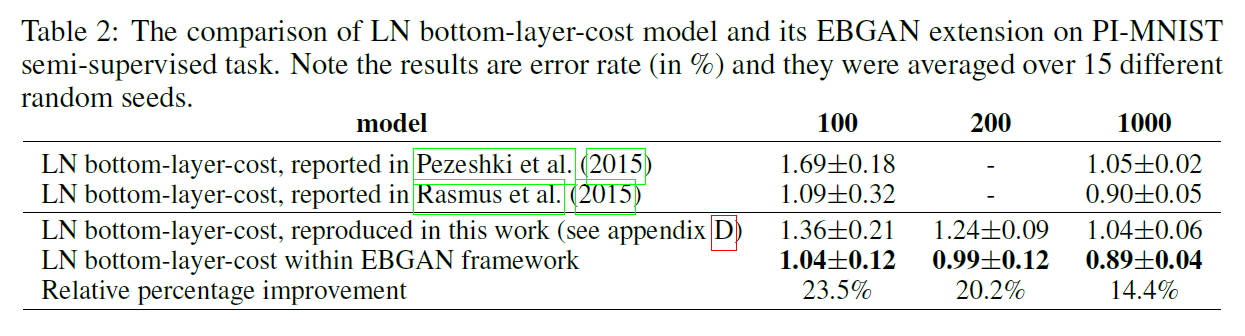
\includegraphics[scale=0.5]{fig/8.png}
  \label{}
\end{figure}
\end{frame}
\begin{frame}{LSUN $\&$ CELEBA}
  \begin{figure}
    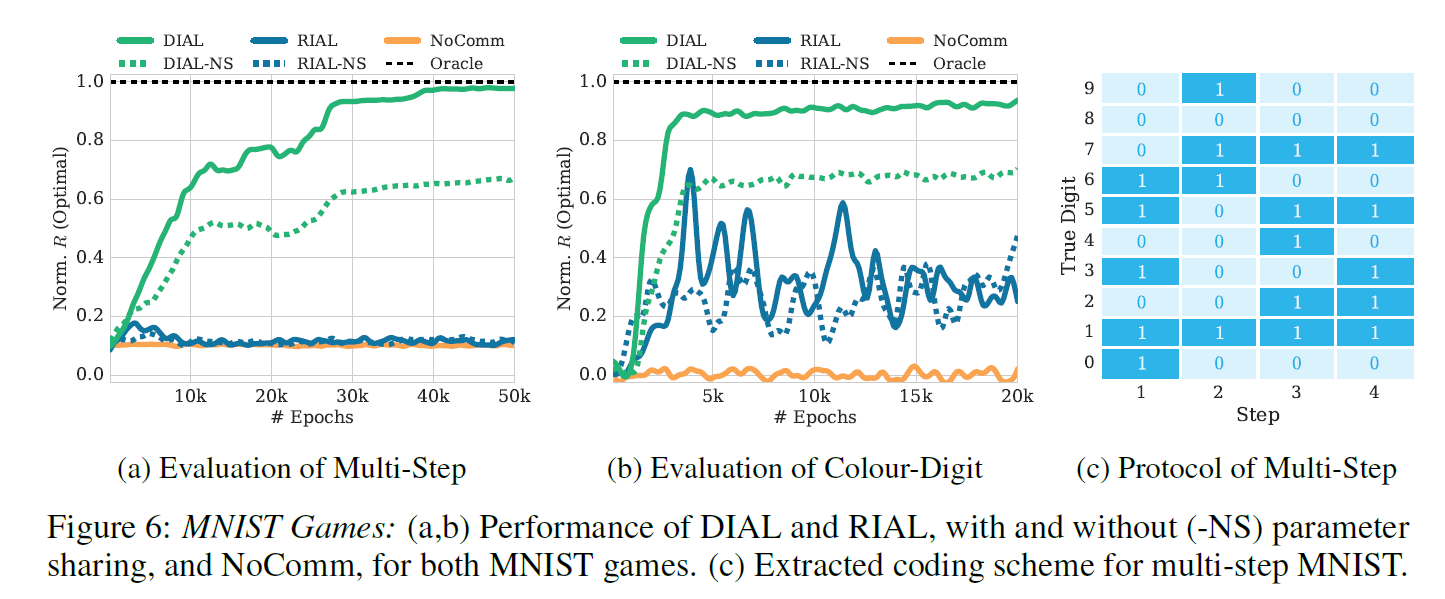
\includegraphics[scale=0.5]{fig/9.png}
    \label{}
  \end{figure}
\end{frame}
\begin{frame}{LSUN $\&$ CELEBA}
  \begin{figure}
    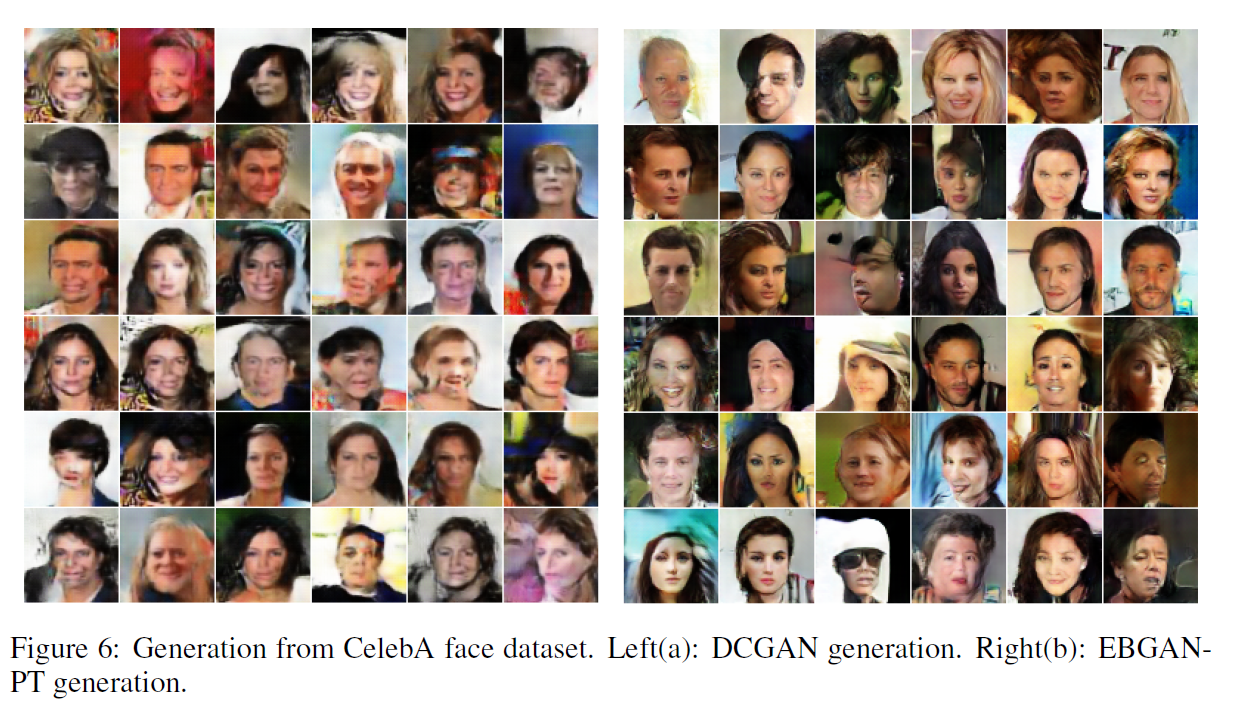
\includegraphics[scale=0.5]{fig/10.png}
    \label{}
  \end{figure}
\end{frame}
\begin{frame}{Imagenet}
  \begin{figure}
    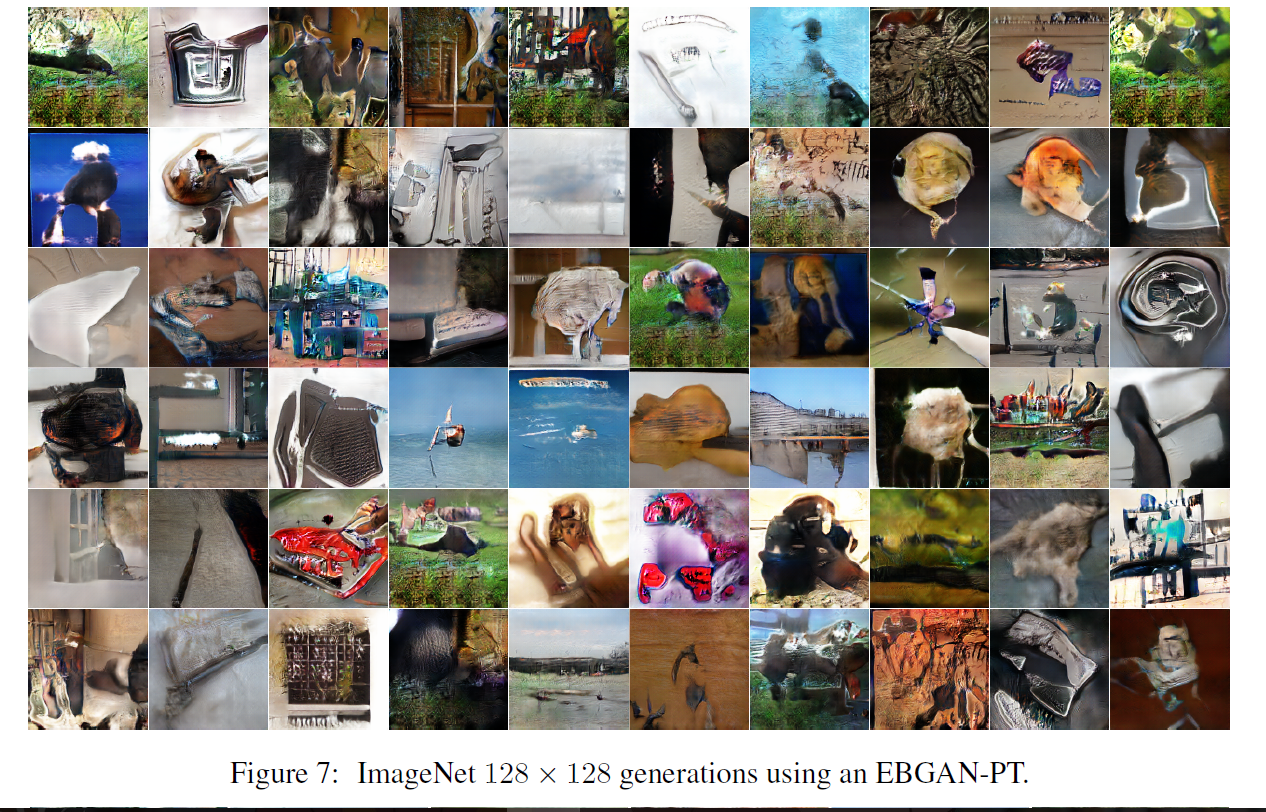
\includegraphics[scale=0.5]{fig/11.png}
    \label{}
  \end{figure}
\end{frame}
\begin{frame}{Imagenet}
  \begin{figure}
    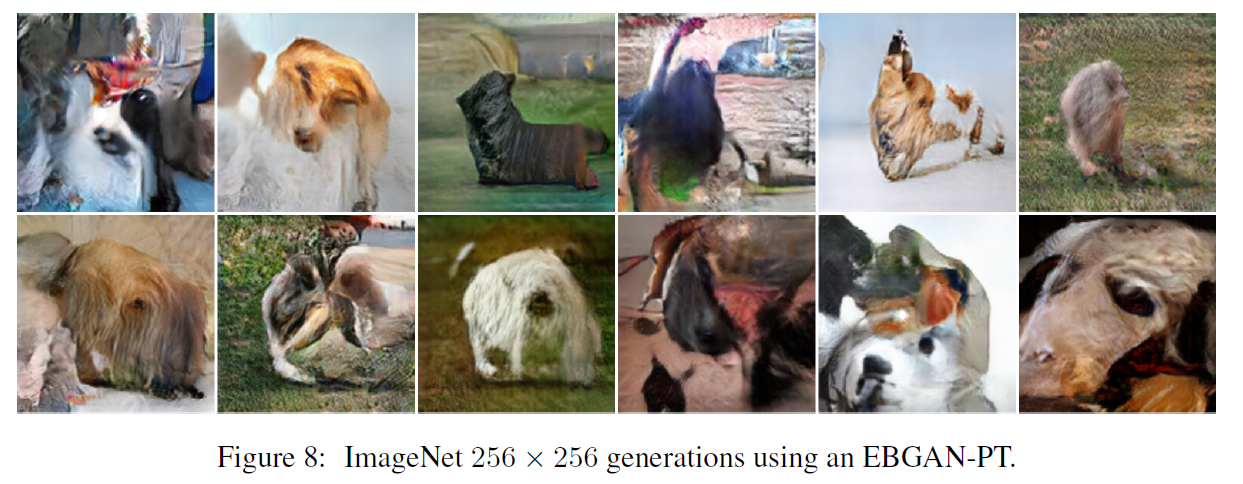
\includegraphics[scale=0.5]{fig/12.png}
    \label{}
  \end{figure}
\end{frame}
\section{Reference}
\begin{frame}{Reference}
  Reference:

  [1] J Zhao,M Mathieu,Y Lecun; Energy-based Generative Adversarial Network
\end{frame}
\end{document}
